\documentclass[sigconf]{acmart}

\usepackage{booktabs} % For formal tables
\usepackage{graphicx}
\usepackage{rotating}
\usepackage{tabularx}
\usepackage{xstring} % for string operations
\usepackage{wasysym} % Table legend with symbols input from post-processing
\usepackage{MnSymbol} % Table legend with symbols input from post-processing
\usepackage{float}

% define some COCO/dvipsnames colors
\definecolor{Gray}{gray}{0.6}
\definecolor{NavyBlue}{rgb}{0.0, 0.0, 0.5}
\definecolor{Magenta}{rgb}{1.0, 0.0, 1.0}
\definecolor{Black}{rgb}{0.0, 0.0, 0.0}

%%%%%%%%%%%%%%%%%%%%%%%%%%%%%%%%%%%%%%%%%%%%%%%%%%%%%%
% Packages
%\usepackage{graphicx}
%\usepackage[dvipsnames]{xcolor}
%\usepackage{float}
%\usepackage{xstring} % for string operations
%\usepackage{wasysym} % Table legend with symbols input from post-processing
%\usepackage{MnSymbol} % Table legend with symbols input from post-processing
%\usepackage[colorlinks=true, linkcolor=blue]{hyperref} % make COCO papers clickable




% Copyright
%\setcopyright{none}
%\setcopyright{acmcopyright}
%\setcopyright{acmlicensed}
\setcopyright{rightsretained}
%\setcopyright{usgov}
%\setcopyright{usgovmixed}
%\setcopyright{cagov}
%\setcopyright{cagovmixed}


% DOI
\acmDOI{10.475/123_4}

% ISBN
\acmISBN{123-4567-24-567/08/06}

%Conference
\acmConference[GECCO '17]{the Genetic and Evolutionary Computation Conference 2017}{July 15--19, 2017}{Berlin, Germany}
\acmYear{2017}
\copyrightyear{2017}

\acmPrice{15.00}



%%%%%%%%%%%%%%%%%%%%%%   END OF PREAMBLE   %%%%%%%%%%%%%%%%%%%%%%%%%%%%%%%%%%%%

%%%%%%%%%%%%%%%%%%%%%%%%%%%%%%%%%%%%%%%%%%%%%%%%%%%%%%%%%%%%%%%%%%%%%%%%%%%%%%%
%%%%%%%%% TO BE EDITED %%%%%%%%%%%%%%%%%%%%%%%%%%%%%%%%%%%%%%%%%%%%%%%%%%%%%%%%
%%%%%%%%%%%%%%%%%%%%%%%%%%%%%%%%%%%%%%%%%%%%%%%%%%%%%%%%%%%%%%%%%%%%%%%%%%%%%%%
% specify acronyms for algorithm1 (1st arg. of post-processing) and algorithm2 (2nd arg.) 
%\newcommand{\algorithmA}{algorithmB}  % first argument in the post-processing
%\newcommand{\algorithmB}{algorithmB}  % second argument in the post-processing
% for the short acronyms in the tables, adjust the following to lines if required.
%\newcommand{\algorithmAshort}{algA}  % first argument in the post-processing
%\newcommand{\algorithmBshort}{algB}  % second argument in the post-processing

% rungeneric.py writes data into a subfolder of ppdata
\newcommand{\bbobdatapath}{ppdata/} % change default output folder of COCO if desired
\input{\bbobdatapath cocopp_commands.tex} % provide default of algname and algfolder
%%%%%%%%%%%%%%%%%%%%%%%%%%%%%%%%%%%%%%%%%%%%%%%%%%%%%%%%%%%%%%%%%%%%%%%%%%%%%%%
%%%%%%%%%%%%%%%%%%%%%%%%%%%%%%%%%%%%%%%%%%%%%%%%%%%%%%%%%%%%%%%%%%%%%%%%%%%%%%%
%%%%%%%%%%%%%%%%%%%%%%%%%%%%%%%%%%%%%%%%%%%%%%%%%%%%%%%%%%%%%%%%%%%%%%%%%%%%%%%
\graphicspath{{\bbobdatapath\algsfolder}}

% pre-defined commands
\newcommand{\DIM}{\ensuremath{\mathrm{DIM}}}
\newcommand{\aRT}{\ensuremath{\mathrm{aRT}}}
\newcommand{\FEvals}{\ensuremath{\mathrm{FEvals}}}
\newcommand{\nruns}{\ensuremath{\mathrm{Nruns}}}
\newcommand{\Dfb}{\ensuremath{\Delta f_{\mathrm{best}}}}
\newcommand{\Df}{\ensuremath{\Delta f}}
\newcommand{\nbFEs}{\ensuremath{\mathrm{\#FEs}}}
\newcommand{\fopt}{\ensuremath{f_\mathrm{opt}}}
\newcommand{\ftarget}{\ensuremath{f_\mathrm{t}}}
\newcommand{\CrE}{\ensuremath{\mathrm{CrE}}}
\newcommand{\change}[1]{{\color{red} #1}}


\begin{document}

\title{Black-Box Optimization Benchmarking Template for the Comparison of Two Algorithms on the Noiseless Testbed}
\renewcommand{\shorttitle}{Black-Box Optimization Benchmarking Template for Two Algorithms}
\titlenote{Submission deadline: March 31st.}
%Camera-ready paper due April 24th.}}
\subtitle{Draft version}



\author{Firstname Lastname}
%\authornote{tba if needed}
%\orcid{1234-5678-9012}
%\affiliation{%
%  \institution{Institute for Clarity in Documentation}
%  \streetaddress{P.O. Box 1212}
%  \city{Dublin} 
%  \state{Ohio} 
%  \postcode{43017-6221}
%}
%\email{trovato@corporation.com}
%
%\author{G.K.M. Tobin}
%\authornote{The secretary disavows any knowledge of this author's actions.}
%\affiliation{%
%  \institution{Institute for Clarity in Documentation}
%  \streetaddress{P.O. Box 1212}
%  \city{Dublin} 
%  \state{Ohio} 
%  \postcode{43017-6221}
%}
%\email{webmaster@marysville-ohio.com}
%
%\author{Lars Th{\o}rv{\"a}ld}
%\authornote{This author is the
%  one who did all the really hard work.}
%\affiliation{%
%  \institution{The Th{\o}rv{\"a}ld Group}
%  \streetaddress{1 Th{\o}rv{\"a}ld Circle}
%  \city{Hekla} 
%  \country{Iceland}}
%\email{larst@affiliation.org}
%
%\author{Lawrence P. Leipuner}
%\affiliation{
%  \institution{Brookhaven Laboratories}
%  \streetaddress{P.O. Box 5000}}
%\email{lleipuner@researchlabs.org}
%
%\author{Sean Fogarty}
%\affiliation{%
%  \institution{NASA Ames Research Center}
%  \city{Moffett Field}
%  \state{California} 
%  \postcode{94035}}
%\email{fogartys@amesres.org}
%
%\author{Charles Palmer}
%\affiliation{%
%  \institution{Palmer Research Laboratories}
%  \streetaddress{8600 Datapoint Drive}
%  \city{San Antonio}
%  \state{Texas} 
%  \postcode{78229}}
%\email{cpalmer@prl.com}
%
%\author{John Smith}
%\affiliation{\institution{The Th{\o}rv{\"a}ld Group}}
%\email{jsmith@affiliation.org}
%
%\author{Julius P.~Kumquat}
%\affiliation{\institution{The Kumquat Consortium}}
%\email{jpkumquat@consortium.net}

% The default list of authors is too long for headers}
\renewcommand{\shortauthors}{Firstname Lastname et. al.}


\begin{abstract}
to be written
\end{abstract}


%
% The code below should be generated by the tool at
% http://dl.acm.org/ccs.cfm
% Please copy and paste the code instead of the example below. 
%
 \begin{CCSXML}
<ccs2012>
<concept>
<concept_id>10010147.10010178.10010205.10010208</concept_id>
<concept_desc>Computing methodologies~Continuous space search</concept_desc>
<concept_significance>500</concept_significance>
</concept>
</ccs2012>
\end{CCSXML}

\ccsdesc[500]{Computing methodologies~Continuous space search}


% We no longer use \terms command
%\terms{Algorithms}

% Complete with anything that is needed
\keywords{Benchmarking, Black-box optimization}

\maketitle


% \section{Introduction}
%
% \section{Algorithm Presentation}
%
% \section{Experimental Procedure}
%
%%%%%%%%%%%%%%%%%%%%%%%%%%%%%%%%%%%%%%%%%%%%%%%%%%%%%%%%%%%%%%%%%%%%%%%%%%%%%%%
\section{CPU Timing}
%%%%%%%%%%%%%%%%%%%%%%%%%%%%%%%%%%%%%%%%%%%%%%%%%%%%%%%%%%%%%%%%%%%%%%%%%%%%%%%
% note that the following text is just a proposal and can/should be changed to your needs:
In order to evaluate the CPU timing of the algorithm, we have run the \change{MY-ALGORITHM-NAME} on the  \change{bbob test suite \cite{hansen2010fun}} with restarts for a maximum budget equal to \change{$400 (D + 2)$} function evaluations according to \cite{hansen2016exp}. The \change{C/Java/Python/Matlab/Octave} code was run on a \change{Mac Intel(R) Core(TM) i5-2400S CPU @ 2.50GHz} with \change{1} processor and \change{4} cores \change{and (compile) options xxx}. The time per function evaluation for dimensions 2, 3, 5, 10, 20\change{, 40} equals \change{$x.x$}, \change{$x.x$}, \change{$x.x$}, \change{$xx$}, \change{$xxx$}\change{, and $xxx$} seconds respectively. 

\change{repeat the above for the second algorithm}

%%%%%%%%%%%%%%%%%%%%%%%%%%%%%%%%%%%%%%%%%%%%%%%%%%%%%%%%%%%%%%%%%%%%%%%%%%%%%%%
\section{Results}
%%%%%%%%%%%%%%%%%%%%%%%%%%%%%%%%%%%%%%%%%%%%%%%%%%%%%%%%%%%%%%%%%%%%%%%%%%%%%%%

Results from experiments according to \cite{hansen2016exp} and \cite{hansen2016perfass} on the benchmark
functions given in \cite{wp200901_2010,hansen2010fun} are presented in
Figures~\ref{fig:scaling}, \ref{fig:scatterplots} and \ref{fig:RLDs} and
in Table~\ref{tab:aRTs}. The experiments were performed with COCO \cite{hansen2016cocoplat},
version \change{2.0}, the plots were produced with version \change{2.0}.

The \textbf{average runtime (aRT)}, used in the figures and table, depends on a
given target function value, $\ftarget=\fopt+\Df$, and is computed over all relevant trials
as the number of function evaluations executed during each trial while the best
function value did not reach \ftarget, summed over all trials
and divided by the number of trials that actually reached \ftarget\
\cite{hansen2010exp,price1997dev}.
\textbf{Statistical significance} is tested with the rank-sum test for a given
target $\Delta\ftarget$ ($10^{-8}$ as in Figure~\ref{fig:scaling}) using,
for each trial, either the number of needed function evaluations to reach
$\Delta\ftarget$ (inverted and multiplied by $-1$), or, if the target was not
reached, the best $\Df$-value achieved, measured only up to the smallest number
of overall function evaluations for any unsuccessful trial under consideration.


%%%%%%%%%%%%%%%%%%%%%%%%%%%%%%%%%%%%%%%%%%%%%%%%%%%%%%%%%%%%%%%%%%%%%%%%%%%%%%%
%%%%%%%%%%%%%%%%%%%%%%%%%%%%%%%%%%%%%%%%%%%%%%%%%%%%%%%%%%%%%%%%%%%%%%%%%%%%%%%

% Scaling of aRT with dimension

%%%%%%%%%%%%%%%%%%%%%%%%%%%%%%%%%%%%%%%%%%%%%%%%%%%%%%%%%%%%%%%%%%%%%%%%%%%%%%%
\begin{figure*}
\centering
\begin{tabular}{@{}c@{}c@{}c@{}c@{}}
\includegraphics[width=0.24\textwidth]{ppfigs_f001}&
\includegraphics[width=0.24\textwidth]{ppfigs_f002}&
\includegraphics[width=0.24\textwidth]{ppfigs_f003}&
\includegraphics[width=0.24\textwidth]{ppfigs_f004}\\[-0.25em]
\includegraphics[width=0.24\textwidth]{ppfigs_f005}&
\includegraphics[width=0.24\textwidth]{ppfigs_f006}&
\includegraphics[width=0.24\textwidth]{ppfigs_f007}&
\includegraphics[width=0.24\textwidth]{ppfigs_f008}\\[-0.25em]
\includegraphics[width=0.24\textwidth]{ppfigs_f009}&
\includegraphics[width=0.24\textwidth]{ppfigs_f010}&
\includegraphics[width=0.24\textwidth]{ppfigs_f011}&
\includegraphics[width=0.24\textwidth]{ppfigs_f012}\\[-0.25em]
\includegraphics[width=0.24\textwidth]{ppfigs_f013}&
\includegraphics[width=0.24\textwidth]{ppfigs_f014}&
\includegraphics[width=0.24\textwidth]{ppfigs_f015}&
\includegraphics[width=0.24\textwidth]{ppfigs_f016}\\[-0.25em]
\includegraphics[width=0.24\textwidth]{ppfigs_f017}&
\includegraphics[width=0.24\textwidth]{ppfigs_f018}&
\includegraphics[width=0.24\textwidth]{ppfigs_f019}&
\includegraphics[width=0.24\textwidth]{ppfigs_f020}\\[-0.25em]
\includegraphics[width=0.24\textwidth]{ppfigs_f021}&
\includegraphics[width=0.24\textwidth]{ppfigs_f022}&
\includegraphics[width=0.24\textwidth]{ppfigs_f023}&
\includegraphics[width=0.24\textwidth]{ppfigs_f024}
\end{tabular}
\vspace*{-0.3cm}
\caption[Expected running time divided by dimension versus dimension]{
\label{fig:scaling}
\bbobppfigslegend{$f_1$ and $f_{24}$}.  % note: \algorithmA and \algorithmB can be defined above
}
% 
\end{figure*}



%%%%%%%%%%%%%%%%%%%%%%%%%%%%%%%%%%%%%%%%%%%%%%%%%%%%%%%%%%%%%%%%%%%%%%%%%%%%%%%
%%%%%%%%%%%%%%%%%%%%%%%%%%%%%%%%%%%%%%%%%%%%%%%%%%%%%%%%%%%%%%%%%%%%%%%%%%%%%%%
 
% Scatter plots per function.

%%%%%%%%%%%%%%%%%%%%%%%%%%%%%%%%%%%%%%%%%%%%%%%%%%%%%%%%%%%%%%%%%%%%%%%%%%%%%%%

%%%%%%%%%%%%%%%%%%%%%%%%%%%%%%%%%%%%%%%%%%%%%%%%%%%%%%%%%%%%%%%%%%%%%%%%%%%%%%%
%%%%%%%%%%%%%%%%%%%%%%%%%%%%%%%%%%%%%%%%%%%%%%%%%%%%%%%%%%%%%%%%%%%%%%%%%%%%%%%
\newcommand{\rot}[2][2.5]{
  \hspace*{-3.5\baselineskip}%
  \begin{rotate}{90}\hspace{#1em}#2
  \end{rotate}}
%%%%%%%%%%%%%%%%%%%%%%%%%%%%%%%%%%%%%%%%%%%%%%%%%%%%%%%%%%%%%%%%%%%%%%%%%%%%%%%
%%%%%%%%%%%%%%%%%%%%%%%%%%%%%%%%%%%%%%%%%%%%%%%%%%%%%%%%%%%%%%%%%%%%%%%%%%%%%%%

\begin{figure*}
\begin{tabular}{*{4}{@{}c@{}}}
    \includegraphics[height=0.2\textwidth]{ppscatter_f001}&
    \includegraphics[height=0.2\textwidth]{ppscatter_f002}&
    \includegraphics[height=0.2\textwidth]{ppscatter_f003}&
    \includegraphics[height=0.2\textwidth]{ppscatter_f004}\\[-0.6em]
    \includegraphics[height=0.2\textwidth]{ppscatter_f005}&
    \includegraphics[height=0.2\textwidth]{ppscatter_f006}&
    \includegraphics[height=0.2\textwidth]{ppscatter_f007}&
    \includegraphics[height=0.2\textwidth]{ppscatter_f008}\\[-0.6em]
    \includegraphics[height=0.2\textwidth]{ppscatter_f009}&
    \includegraphics[height=0.2\textwidth]{ppscatter_f010}&
    \includegraphics[height=0.2\textwidth]{ppscatter_f011}&
    \includegraphics[height=0.2\textwidth]{ppscatter_f012}\\[-0.6em]
    \includegraphics[height=0.2\textwidth]{ppscatter_f013}&
    \includegraphics[height=0.2\textwidth]{ppscatter_f014}&
    \includegraphics[height=0.2\textwidth]{ppscatter_f015}&
    \includegraphics[height=0.2\textwidth]{ppscatter_f016}\\[-0.6em]
    \includegraphics[height=0.2\textwidth]{ppscatter_f017}&
    \includegraphics[height=0.2\textwidth]{ppscatter_f018}&
    \includegraphics[height=0.2\textwidth]{ppscatter_f019}&
    \includegraphics[height=0.2\textwidth]{ppscatter_f020}\\[-0.6em]
    \includegraphics[height=0.2\textwidth]{ppscatter_f021}&
    \includegraphics[height=0.2\textwidth]{ppscatter_f022}&
    \includegraphics[height=0.2\textwidth]{ppscatter_f023}&
    \includegraphics[height=0.2\textwidth]{ppscatter_f024}
\end{tabular}
\caption{\label{fig:scatterplots}
\bbobppscatterlegend{$f_1$--$f_{24}$}
}
\end{figure*}


%%%%%%%%%%%%%%%%%%%%%%%%%%%%%%%%%%%%%%%%%%%%%%%%%%%%%%%%%%%%%%%%%%%%%%%%%%%%%%%
%%%%%%%%%%%%%%%%%%%%%%%%%%%%%%%%%%%%%%%%%%%%%%%%%%%%%%%%%%%%%%%%%%%%%%%%%%%%%%%
 
% Empirical cumulative distribution functions (ECDFs) per function group.

%%%%%%%%%%%%%%%%%%%%%%%%%%%%%%%%%%%%%%%%%%%%%%%%%%%%%%%%%%%%%%%%%%%%%%%%%%%%%%%
\begin{figure*}
 \begin{tabular}{l@{\hspace*{-0.00\textwidth}}l@{\hspace*{0.01\textwidth}}|l@{\hspace*{-0.00\textwidth}}l}
 \multicolumn{2}{c}{5-D} & \multicolumn{2}{c}{20-D} \\
 \rot[2.9]{all functions}
 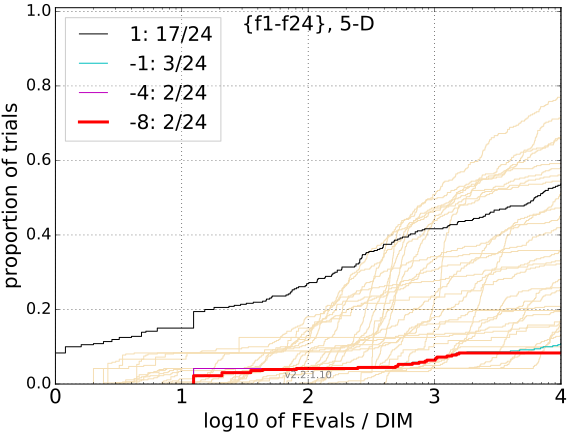
\includegraphics[height=0.14\textheight]{pprldistr_05D_noiselessall} & 
 \includegraphics[height=0.14\textheight]{pplogabs_05D_noiselessall} &
 \includegraphics[height=0.14\textheight]{pprldistr_20D_noiselessall} &
 \includegraphics[height=0.14\textheight]{pplogabs_20D_noiselessall}\\
 \rot[2.7]{separable fcts}
 \includegraphics[height=0.14\textheight]{pprldistr_05D_separ} & 
 \includegraphics[height=0.14\textheight]{pplogabs_05D_separ} &
 \includegraphics[height=0.14\textheight]{pprldistr_20D_separ} &
 \includegraphics[height=0.14\textheight]{pplogabs_20D_separ} \\
 \rot[2.75]{moderate fcts}
 \includegraphics[height=0.14\textheight]{pprldistr_05D_lcond} & 
 \includegraphics[height=0.14\textheight]{pplogabs_05D_lcond} &
 \includegraphics[height=0.14\textheight]{pprldistr_20D_lcond} & 
 \includegraphics[height=0.14\textheight]{pplogabs_20D_lcond}\\
 \rot[1.4]{ill-conditioned fcts}
 \includegraphics[height=0.14\textheight]{pprldistr_05D_hcond} & 
 \includegraphics[height=0.14\textheight]{pplogabs_05D_hcond} &
 \includegraphics[height=0.14\textheight]{pprldistr_20D_hcond} &
 \includegraphics[height=0.14\textheight]{pplogabs_20D_hcond} \\
 \rot[2.1]{multi-modal fcts}
 \includegraphics[height=0.14\textheight]{pprldistr_05D_multi} & 
 \includegraphics[height=0.14\textheight]{pplogabs_05D_multi} &
 \includegraphics[height=0.14\textheight]{pprldistr_20D_multi} &
 \includegraphics[height=0.14\textheight]{pplogabs_20D_multi} \\
 \rot[1.4]{weak structure fcts}
 \includegraphics[height=0.14\textheight]{pprldistr_05D_mult2} & 
 \includegraphics[height=0.14\textheight]{pplogabs_05D_mult2} &
 \includegraphics[height=0.14\textheight]{pprldistr_20D_mult2} & 
 \includegraphics[height=0.14\textheight]{pplogabs_20D_mult2}\\
 \end{tabular}
\vspace*{-0.2cm}
 \caption{\label{fig:RLDs}
 \bbobpprldistrlegendtwo{}
 }
\end{figure*}


%%%%%%%%%%%%%%%%%%%%%%%%%%%%%%%%%%%%%%%%%%%%%%%%%%%%%%%%%%%%%%%%%%%%%%%%%%%%%%%
%%%%%%%%%%%%%%%%%%%%%%%%%%%%%%%%%%%%%%%%%%%%%%%%%%%%%%%%%%%%%%%%%%%%%%%%%%%%%%%
 
% Table showing the average runtime (aRT in number of function
% evaluations) divided by the best aRT measured during BBOB-2009 (given in the
% first row of each cell) for functions $f_1$--$f_{24}$.

%%%%%%%%%%%%%%%%%%%%%%%%%%%%%%%%%%%%%%%%%%%%%%%%%%%%%%%%%%%%%%%%%%%%%%%%%%%%%%%
\begin{table*}
\mbox{\begin{minipage}[t]{0.495\textwidth}
\centering
5-D\\[5pt]
\tiny
\pptablesheader
\input{\bbobdatapath\algsfolder pptables_f001_05D} 

\input{\bbobdatapath\algsfolder pptables_f002_05D}

\input{\bbobdatapath\algsfolder pptables_f003_05D}

\input{\bbobdatapath\algsfolder pptables_f004_05D}

\input{\bbobdatapath\algsfolder pptables_f005_05D}

\input{\bbobdatapath\algsfolder pptables_f006_05D}

\input{\bbobdatapath\algsfolder pptables_f007_05D}

\input{\bbobdatapath\algsfolder pptables_f008_05D}

\input{\bbobdatapath\algsfolder pptables_f009_05D}

\input{\bbobdatapath\algsfolder pptables_f010_05D}

\input{\bbobdatapath\algsfolder pptables_f011_05D}

\input{\bbobdatapath\algsfolder pptables_f012_05D}

\input{\bbobdatapath\algsfolder pptables_f013_05D}

\input{\bbobdatapath\algsfolder pptables_f014_05D}

\input{\bbobdatapath\algsfolder pptables_f015_05D}

\input{\bbobdatapath\algsfolder pptables_f016_05D}

\input{\bbobdatapath\algsfolder pptables_f017_05D}

\input{\bbobdatapath\algsfolder pptables_f018_05D}

\input{\bbobdatapath\algsfolder pptables_f019_05D}

\input{\bbobdatapath\algsfolder pptables_f020_05D}

\input{\bbobdatapath\algsfolder pptables_f021_05D}

\input{\bbobdatapath\algsfolder pptables_f022_05D}

\input{\bbobdatapath\algsfolder pptables_f023_05D}

\input{\bbobdatapath\algsfolder pptables_f024_05D}
\end{tabularx}
\end{minipage}}
\hspace{0.002\textwidth}
\mbox{\begin{minipage}[t]{0.495\textwidth}
\centering
20-D\\[5pt]
\tiny
\pptablesheader
\input{\bbobdatapath\algsfolder pptables_f001_20D} 

\input{\bbobdatapath\algsfolder pptables_f002_20D}

\input{\bbobdatapath\algsfolder pptables_f003_20D}

\input{\bbobdatapath\algsfolder pptables_f004_20D}

\input{\bbobdatapath\algsfolder pptables_f005_20D}

\input{\bbobdatapath\algsfolder pptables_f006_20D}

\input{\bbobdatapath\algsfolder pptables_f007_20D}

\input{\bbobdatapath\algsfolder pptables_f008_20D}

\input{\bbobdatapath\algsfolder pptables_f009_20D}

\input{\bbobdatapath\algsfolder pptables_f010_20D}

\input{\bbobdatapath\algsfolder pptables_f011_20D}

\input{\bbobdatapath\algsfolder pptables_f012_20D}

\input{\bbobdatapath\algsfolder pptables_f013_20D}

\input{\bbobdatapath\algsfolder pptables_f014_20D}

\input{\bbobdatapath\algsfolder pptables_f015_20D}

\input{\bbobdatapath\algsfolder pptables_f016_20D}

\input{\bbobdatapath\algsfolder pptables_f017_20D}

\input{\bbobdatapath\algsfolder pptables_f018_20D}

\input{\bbobdatapath\algsfolder pptables_f019_20D}

\input{\bbobdatapath\algsfolder pptables_f020_20D}

\input{\bbobdatapath\algsfolder pptables_f021_20D}

\input{\bbobdatapath\algsfolder pptables_f022_20D}

\input{\bbobdatapath\algsfolder pptables_f023_20D}

\input{\bbobdatapath\algsfolder pptables_f024_20D}
\end{tabularx}
\end{minipage}}

\caption{\label{tab:aRTs}
\bbobpptablesmanylegend{dimensions $5$ (left) and $20$ (right)}
}
\end{table*}



%%%%%%%%%%%%%%%%%%%%%%%%%%%%%%%%%%%%%%%%%%%%%%%%%%%%%%%%%%%%%%%%%%%%%%%%%%%%%%%

\bibliographystyle{ACM-Reference-Format}
\bibliography{bbob}  % bbob.bib is the name of the Bibliography in this case

\clearpage % otherwise the last figure might be missing



\end{document}

%%%%%%%%%%%%%%%%%%%%%%%%%%%%%%%%%%%%%%%%%%%%%%%%%%%%%%%%%%%%%%%%%%%%%%%%%%%%%%%%%%%%%%%%%%%
